\documentclass[tikz,border=3mm]{standalone}
\usepackage{tikz-feynman}
\begin{document}
 \feynmandiagram [] { 
 	a -- [rmomentum'={[label distance=-1.6pt]\(p_3\)}] b [blob] -- [momentum={[label distance=-1.6pt]\(p_2\)}] c,
	b -- [momentum={[label distance=-1.6pt]\(p_4\)}]d,
	b -- [momentum={[label distance=-1.6pt]\(p_1\)}] e,
	b -- [scalar, momentum={[label distance=-1.6pt]\(p_5\)}] f,
	f -- [momentum=\(q_6\)] g,
	f -- [momentum'=\(q_5\)] h,
	c -- [momentum=\(q_2\)] c1,
	d -- [momentum=\(q_4\)] d1,
	e -- [momentum=\(q_1\)] e1,
	a -- [momentum=\(q_3\)] a1,
};
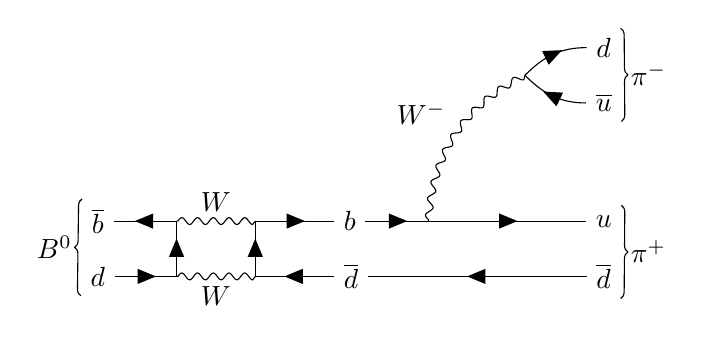
\begin{tikzpicture}
  \begin{feynman}
    \vertex (a1) {\(\overline b\)};
    \vertex[right=1cm of a1] (a2);
    \vertex[right=1cm of a2] (a3);
    \vertex[right=1cm of a3] (a4) {\(b\)};
    \vertex[right=1cm of a4] (a5);
    \vertex[right=2cm of a5] (a6) {\(u\)};

    \vertex[below=2em of a1] (b1) {\(d\)};
    \vertex[right=1cm of b1] (b2);
    \vertex[right=1cm of b2] (b3);
    \vertex[right=1cm of b3] (b4) {\(\overline d\)};
    \vertex[below=2em of a6] (b5) {\(\overline d\)};

    \vertex[above=of a6] (c1) {\(\overline u\)};
    \vertex[above=2em of c1] (c3) {\(d\)};
    \vertex at ($(c1)!0.5!(c3) - (1cm, 0)$) (c2);

    \diagram* {
      {[edges=fermion]
        (b1) -- (b2) -- (a2) -- (a1),
        (b5) -- (b4) -- (b3) -- (a3) -- (a4) -- (a5) -- (a6),
      },
      (a2) -- [boson, edge label=\(W\)] (a3),
      (b2) -- [boson, edge label'=\(W\)] (b3),

      (c1) -- [fermion, out=180, in=-45] (c2) -- [fermion, out=45, in=180] (c3),
      (a5) -- [boson, bend left, edge label=\(W^{-}\)] (c2),
    };

    \draw [decoration={brace}, decorate] (b1.south west) -- (a1.north west)
          node [pos=0.5, left] {\(B^{0}\)};
    \draw [decoration={brace}, decorate] (c3.north east) -- (c1.south east)
          node [pos=0.5, right] {\(\pi^{-}\)};
    \draw [decoration={brace}, decorate] (a6.north east) -- (b5.south east)
          node [pos=0.5, right] {\(\pi^{+}\)};
  \end{feynman}
\end{tikzpicture}
\end{document}